%%%%%%%%%%%%%%%%%%%%%%%%%%%%%%%%%%%%%%%%%%%%%%%%%%%%%%%%%%%%%%%%%%%%%%%%%%%%%%%%
%2345678901234567890123456789012345678901234567890123456789012345678901234567890
%        1         2         3         4         5         6         7         8

\documentclass[letterpaper, 10 pt, conference]{ieeeconf}  % Comment this line out if you need a4paper

%\documentclass[a4paper, 10pt, conference]{ieeeconf}      % Use this line for a4 paper

%% \IEEEoverridecommandlockouts                              % This command is only needed if
                                                          % you want to use the \thanks command

\overrideIEEEmargins                                      % Needed to meet printer requirements.

% See the \addtolength command later in the file to balance the column lengths
% on the last page of the document

% The following packages can be found on http:\\www.ctan.org
%\usepackage{graphics} % for pdf, bitmapped graphics files
%\usepackage{epsfig} % for postscript graphics files
%\usepackage{mathptmx} % assumes new font selection scheme installed
%\usepackage{times} % assumes new font selection scheme installed
%\usepackage{amsmath} % assumes amsmath package installed
%\usepackage{amssymb}  % assumes amsmath package installed
\usepackage [vscale=0.76,includehead]{geometry}
\usepackage{graphicx}
\usepackage{amsmath}
\usepackage{array}
\usepackage{fullpage}
\usepackage{mathptmx} % font = times
\usepackage{helvet} % font sf = helvetica
\usepackage[latin1]{inputenc}
\usepackage{relsize}
\usepackage{graphicx}
\usepackage{caption}
\usepackage{subcaption}

\usepackage{pgfplots}
\newcommand{\rot}[2]{\ensuremath{C_{\,#1}^{\,#2}}}
\definecolor{amethyst}{rgb}{0.5, 0.3, 0.7}

% and optionally (as of Pgfplots 1.3):
\pgfplotsset{compat=newest}
\pgfplotsset{plot coordinates/math parser=false}

\title{\LARGE \bf
Absolute scale velocity determination combining visual and inertial measurements for micro aerial vehicles
}


\author{Jacques Kaiser and Agostino Martinelli% <-this % stops a space
%% \thanks{*This work was not supported by any organization}% <-this % stops a space
%% \thanks{$^{1}$Albert Author is with Faculty of Electrical Engineering, Mathematics and Computer Science,
%%         University of Twente, 7500 AE Enschede, The Netherlands
%%         {\tt\small albert.author@papercept.net}}%
%% \thanks{$^{2}$Bernard D. Researcheris with the Department of Electrical Engineering, Wright State University,
%%         Dayton, OH 45435, USA
%%         {\tt\small b.d.researcher@ieee.org}}%
}


\begin{document}



\maketitle
\thispagestyle{empty}
\pagestyle{empty}


%%%%%%%%%%%%%%%%%%%%%%%%%%%%%%%%%%%%%%%%%%%%%%%%%%%%%%%%%%%%%%%%%%%%%%%%%%%%%%%%
\begin{abstract}

Hi

\end{abstract}


%%%%%%%%%%%%%%%%%%%%%%%%%%%%%%%%%%%%%%%%%%%%%%%%%%%%%%%%%%%%%%%%%%%%%%%%%%%%%%%%

\section{INTRODUCTION}




Autonomous mobile robots navigating in unknow environments have an intrinsic need to perform localization and mapping using only on-board sensors.
Concerning Micro Aerial Vehicles (MAV), a critical issue is to limit the number of on-board sensors to reduce weight and power consumption.
Therefore, a common setup is to combine a monocular camera with an inertial measurements unit (IMU).
On top of being cheap, these sensors have very interesting complementarities.
Additionaly, they can operate in indoor environments where Global Positioning System (GPS) signals are shadowed.
An open question is how to optimally fuse the information provided by these sensors.

Currently, most sensor fusion algorithms are either filter based or iterative. That is, given a current state and measurements, they return an updated state.
While working well in practice, these algorithms need to be provided by an external initial state.

The initialization of a filter based method is critical.
Due to non-linearity of the system, a poor initialization can result into converging towards local minima and  providing faulty states with high confidence.
Indeed, another shortcoming of filters is that they can silently fail.

In this work we demonstrate the efficiency of a recent closed-form solution introduced in \cite{Martinelli2012}\cite{Martinelli2014} that fuses visual and inertial data to obtain the structure of the environment at the global scale along with the attitude and the speed of the robot.

By nature, a closed-form solution is deterministic and thus does not require any initialization.
It is assumed that the camera is calibrated and the transformation between the IMU and the camera is known.
This is a fair assumption for industrial drones to come pre-calibrated.

In this work, we have studied the recent closed-form solution proposed by \cite{Martinelli2014} that performs visual-inertial sensor fusion without requiring an initialization.
We implemented this method in order to test it with real terrain data.
This allowed us to identify its bottlenecks and bring modifications to overcome them.

Specifically, we started by reformulating the equations for greater numerical stability.
This lead to a major leap in the quality of the estimations.

We then investigated the impact of biased inertial measurements.
Despite the case of biased accelerometer was originally studied in \cite{Martinelli2014} we show that its low impact on the system makes it hard to estimate.

One major bottleneck of this method was the impact of biased gyroscope measurements.
In other words, the performance becomes very poor in presence of a bias on the gyroscope and, in practice, the overall method could only be successfully used with a very precise - and expensive - gyroscope.
We then introduced a simple method that automatically estimates this bias.

However, this method requires a significant amount of data to provide correct estimates of the gyroscope bias (either many features or long time of integration).
We were able to get rid of this limitation with a simple statistical trick by adding a regularization term to our cost function.
%tweak in the cost function we are minimizing.

By adding this new method for the bias estimation to the original method we obtain results which are equivalent to the ones in absence of bias.
Compared to the original method, the new method is now robust to the gyroscope bias, and also provides the gyroscope bias.
%% Specifically, this method can accurately estimate the initial speed, the gravity, the distance to the features and the gyroscope bias for very short time of integration (around 2 seconds) and low amount of observed point-features (around 5).


%% \begin{figure}[h!]
%%         \centering
%%    \resizebox{0.4\textwidth}{!}{\input{./graph}}
%%         \caption{Estimation error of the original formulation of the Closed-Form solution against the improved Closed-Form solution observing 7 features over 3 seconds.}
%% \end{figure}

\section{RELATED WORK}
\section{THE CLOSED-FORM SOLUTION}

In this paper, we do not provide a new derivation of the  closed-form solution.
Instead, we consider the latest derivation proposed in \cite{Martinelli2014}.
Specifically, the author expresses the state of the MAV with respect to the visual and inertial measurements in Equation \ref{eq:final1}:


\begin{equation} \tag{6} \label{eq:final1}
S_j = \lambda_1^i\mu_1^i - V t_j - G \frac{t_j^2}{2} - \lambda^i_j \mu^i_j
\end{equation}
With:
\begin{itemize}
\item $\mu_j^i$ the normalized bearing of point-feature $i$ at time $t_j$ in the initial local frame;
\item $\lambda_j^i$ the distance to the point-feature $i$ at time $t_j$;
\item $V$ the initial velocity in the initial local frame;
\item $G$ the initial gravity in the initial local frame;
\item $S_j$ the integration up to time $t_j$ of the rotated linear acceleration data.
\end{itemize}

\begin{figure}[h!]
  \centering
  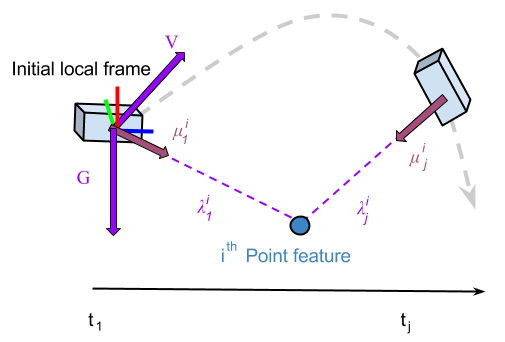
\includegraphics[width=0.90\columnwidth]{images/closedFormExplained}
  \caption{Visual representation of Equation \ref{eq:final1}.
  The unknowns of the equation are colored in \textcolor{amethyst}{purple}.}
\end{figure}


The unknowns of Equation \ref{eq:final1} are the distances $\lambda_j^i$ and the vectors $V$ and $G$.
Note that the knowledge of $G$ is equivalent to the knowledge of the roll and pitch angles.
The vectors $\mu_j^i$ are fully determined by camera observations and gyroscope measurements,
and the vectors $S_j$ are determined by accelerometer and gyroscope measurements.

As Equation \ref{eq:final1} holds for each three dimensions of all point-features $i=1,...,N$ and each observation starting from the second one $j=2,...n_i$, we therefore have a system consisting of $3(n_i-1)N$ equations in $6 + Nn_i$ unknowns.
Indeed, note that when the first observation occurs, at $t_j = 0$, Equation \ref{eq:final1} is always satisfied thus does not provide information.
We can write our system using matrix notations. Solving the system is equivalent to inverting a matrix of $3(n_i-1)N$ rows and $6+Nn_i$ columns.

In \cite{Martinelli2014}, the author proceeded to one more step before expressing the underlying linear system.
For an observation at time $t_j$, the equation of the first point-feature $i=1$ happening at time $t_j$ is subtracted to all other point-features $1<i<=N$ at time $t_j$ (Equation 7).
This additional step has the effect to corrupt all measurements with the first measurement,
hence worsening the performance of the closed-form solution.
In this paper, we do not take to this additional step.

The linear system in Equation \ref{eq:final1} can be written in the following compact format:

\begin{equation}
\label{eq:mat1}
\Xi X = S
\end{equation}

The matrix $\Xi$ and the vector $S$ are fully determined by the measurements, while $X$ is the unknown vector.
More specifically:

\[
S \equiv [S_2^T, ...,S_2^T, S_3^T,...,S_3^T,...,S_{n_i}^T,...,S_{n_i}^T]^T
\]
\[
X \equiv [ G^T, V^T, \lambda_1^1, ..., \lambda_1^N, ..., \lambda_{n_i}^1, ..., \lambda_{n_i}^N]^T \\
\]

\begin{multline}
  \Xi \equiv \\
  \left[
    {\scriptscriptstyle
    \begin{array}{l|l|l|l|l|l|l|l|l|l|l}
      T_2 & S_2 & \mu_1^1 & 0_3 & 0_3 & -\mu_2^1 & 0_3 & 0_3 & 0_3 & 0_3 & 0_3 \\
      T_2 & S_2 & 0_3 & \mu_1^2 & 0_3 & 0_3 & -\mu_2^2 & 0_3 & 0_3 & 0_3 & 0_3 \\
      ... & ... & ... & ... & ... & ... & ... & ... & ... & ... & ... \\
      T_2 & S_2 & 0_3 & 0_3 & \mu_1^N & 0_3 & 0_3 & -\mu_2^N & 0_3 & 0_3 & 0_3 \\
      ... & ... & ... & ... & ... & ... & ... & ... & ... & ... & ... \\
      ... & ... & ... & ... & ... & ... & ... & ... & ... & ... & ... \\
      T_{n_i} & S_{n_i} & \mu_1^1 & 0_3 & 0_3 & 0_3 & 0_3 & 0_3 & -\mu_{n_i}^1 & 0_3 & 0_3 \\
      T_{n_i} & S_{n_i} & 0_3 & \mu_1^2 & 0_3 & 0_3 & 0_3 & 0_3 & 0_3 & -\mu_{n_i}^2 & 0_3 \\
      ... & ... & ... & ... & ... & ... & ... & ... & ... & ... & ... \\
      T_{n_i} & S_{n_i} & 0_3 & 0_3 & \mu_1^N & 0_3 & 0_3 & 0_3 & 0_3 & 0_3 & -\mu_{n_i}^N
    \end{array}
    }
    \right]
\end{multline}


Where $T_j \equiv - \frac{t^2_j}{2} I_3$, $S_j \equiv -t_j I_3$ and $I_3$ is the identity 3 x 3 matrix; $0_{33}$ is the 3 x 3 zero matrix.
Note that the matrix $\Xi$ and the vector $S$ are different from the one proposed in \cite{Martinelli2014}.
This is due to the additional step we did not take for numerical stability reasons.

We can therefore recover the initial velocity, the roll and pitch angles and the distances to the point-features
by finding the vector $X$ which satisfies \ref{eq:final1}.


%% The system therefore becomes:

%% \begin{equation} \label{eq:final2}
%% \left[
%% \begin{array}{lcl}
%% S_j &=& \lambda_1^i\mu_1^i - V t_j - G \frac{t_j^2}{2} - \lambda^i_j \mu^i_j\\
%% 0_3 &=& \lambda_1^1\mu_1^1 - \lambda_j^1\mu_j^1 - \lambda_1^i\mu_1^i + \lambda^i_j \mu^i_j
%% \end{array}
%% \right.
%% \end{equation}



\section{PERFORMANCE BOTTLENECKS}
\section{ESTIMATING THE GYROSCOPE BIAS}
\section{RESULTS}
\section{CONCLUSION}


\bibliographystyle{plain}
\bibliography{library}

\end{document}
